% =============================================================================#
% created by Kevin Horton, 2011
% 
% This file is part of ft_program.
% 
%     ft_program is free software: The exectuable files are licensed under the
%     Gnu Public License, but the latex files, including this file, are placed 
%     in the public domain.  
%
% =============================================================================#
% GNUPLOT: LaTeX picture with Postscript
\begingroup
  \makeatletter
  \providecommand\color[2][]{%
    \GenericError{(gnuplot) \space\space\space\@spaces}{%
      Package color not loaded in conjunction with
      terminal option `colourtext'%
    }{See the gnuplot documentation for explanation.%
    }{Either use 'blacktext' in gnuplot or load the package
      color.sty in LaTeX.}%
    \renewcommand\color[2][]{}%
  }%
  \providecommand\includegraphics[2][]{%
    \GenericError{(gnuplot) \space\space\space\@spaces}{%
      Package graphicx or graphics not loaded%
    }{See the gnuplot documentation for explanation.%
    }{The gnuplot epslatex terminal needs graphicx.sty or graphics.sty.}%
    \renewcommand\includegraphics[2][]{}%
  }%
  \providecommand\rotatebox[2]{#2}%
  \@ifundefined{ifGPcolor}{%
    \newif\ifGPcolor
    \GPcolorfalse
  }{}%
  \@ifundefined{ifGPblacktext}{%
    \newif\ifGPblacktext
    \GPblacktexttrue
  }{}%
  % define a \g@addto@macro without @ in the name:
  \let\gplgaddtomacro\g@addto@macro
  % define empty templates for all commands taking text:
  \gdef\gplbacktext{}%
  \gdef\gplfronttext{}%
  \makeatother
  \ifGPblacktext
    % no textcolor at all
    \def\colorrgb#1{}%
    \def\colorgray#1{}%
  \else
    % gray or color?
    \ifGPcolor
      \def\colorrgb#1{\color[rgb]{#1}}%
      \def\colorgray#1{\color[gray]{#1}}%
      \expandafter\def\csname LTw\endcsname{\color{white}}%
      \expandafter\def\csname LTb\endcsname{\color{black}}%
      \expandafter\def\csname LTa\endcsname{\color{black}}%
      \expandafter\def\csname LT0\endcsname{\color[rgb]{1,0,0}}%
      \expandafter\def\csname LT1\endcsname{\color[rgb]{0,1,0}}%
      \expandafter\def\csname LT2\endcsname{\color[rgb]{0,0,1}}%
      \expandafter\def\csname LT3\endcsname{\color[rgb]{1,0,1}}%
      \expandafter\def\csname LT4\endcsname{\color[rgb]{0,1,1}}%
      \expandafter\def\csname LT5\endcsname{\color[rgb]{1,1,0}}%
      \expandafter\def\csname LT6\endcsname{\color[rgb]{0,0,0}}%
      \expandafter\def\csname LT7\endcsname{\color[rgb]{1,0.3,0}}%
      \expandafter\def\csname LT8\endcsname{\color[rgb]{0.5,0.5,0.5}}%
    \else
      % gray
      \def\colorrgb#1{\color{black}}%
      \def\colorgray#1{\color[gray]{#1}}%
      \expandafter\def\csname LTw\endcsname{\color{white}}%
      \expandafter\def\csname LTb\endcsname{\color{black}}%
      \expandafter\def\csname LTa\endcsname{\color{black}}%
      \expandafter\def\csname LT0\endcsname{\color{black}}%
      \expandafter\def\csname LT1\endcsname{\color{black}}%
      \expandafter\def\csname LT2\endcsname{\color{black}}%
      \expandafter\def\csname LT3\endcsname{\color{black}}%
      \expandafter\def\csname LT4\endcsname{\color{black}}%
      \expandafter\def\csname LT5\endcsname{\color{black}}%
      \expandafter\def\csname LT6\endcsname{\color{black}}%
      \expandafter\def\csname LT7\endcsname{\color{black}}%
      \expandafter\def\csname LT8\endcsname{\color{black}}%
    \fi
  \fi
  \setlength{\unitlength}{0.0500bp}%
  \begin{picture}(5760.00,5040.00)%
    \gplgaddtomacro\gplbacktext{%
      \csname LTb\endcsname%
      \put(1210,704){\makebox(0,0)[r]{\strut{} 1100}}%
      \put(1210,1156){\makebox(0,0)[r]{\strut{} 1200}}%
      \put(1210,1609){\makebox(0,0)[r]{\strut{} 1300}}%
      \put(1210,2061){\makebox(0,0)[r]{\strut{} 1400}}%
      \put(1210,2513){\makebox(0,0)[r]{\strut{} 1500}}%
      \put(1210,2966){\makebox(0,0)[r]{\strut{} 1600}}%
      \put(1210,3418){\makebox(0,0)[r]{\strut{} 1700}}%
      \put(1210,3870){\makebox(0,0)[r]{\strut{} 1800}}%
      \put(1210,4323){\makebox(0,0)[r]{\strut{} 1900}}%
      \put(1210,4775){\makebox(0,0)[r]{\strut{} 2000}}%
      \put(1342,484){\makebox(0,0){\strut{} 78}}%
      \put(1751,484){\makebox(0,0){\strut{} 79}}%
      \put(2159,484){\makebox(0,0){\strut{} 80}}%
      \put(2568,484){\makebox(0,0){\strut{} 81}}%
      \put(2977,484){\makebox(0,0){\strut{} 82}}%
      \put(3386,484){\makebox(0,0){\strut{} 83}}%
      \put(3794,484){\makebox(0,0){\strut{} 84}}%
      \put(4203,484){\makebox(0,0){\strut{} 85}}%
      \put(4612,484){\makebox(0,0){\strut{} 86}}%
      \put(5020,484){\makebox(0,0){\strut{} 87}}%
      \put(5429,484){\makebox(0,0){\strut{} 88}}%
      \put(308,2739){\rotatebox{-270}{\makebox(0,0){\strut{}Weight (lb)}}}%
      \put(3385,154){\makebox(0,0){\strut{}CG (inches aft of datum)}}%
      \put(1751,3735){\makebox(0,0)[l]{\strut{}\ding{172}}}%
      \put(1751,2604){\makebox(0,0)[l]{\strut{}\ding{173}}}%
      \put(4714,3735){\makebox(0,0)[l]{\strut{}\ding{174}}}%
      \put(1342,-651){\makebox(0,0)[l]{\strut{}\ding{172} Restricted Aerobatic Weight/CG Envelope}}%
      \put(1342,-968){\makebox(0,0)[l]{\strut{}\ding{173} Aerobatic Weight/CG Envelope}}%
      \put(1342,-1284){\makebox(0,0)[l]{\strut{}\ding{174} Normal Weight/CG Envelope}}%
    }%
    \gplgaddtomacro\gplfronttext{%
      \put(4442,4602){\makebox(0,0)[r]{\strut{}Fuel Burn}}%
      \put(2328,3214){\makebox(0,0)[l]{\strut{}Start}}%
      \put(2351,2047){\makebox(0,0)[l]{\strut{}Zero Fuel}}%
    }%
    \gplbacktext
    \put(0,0){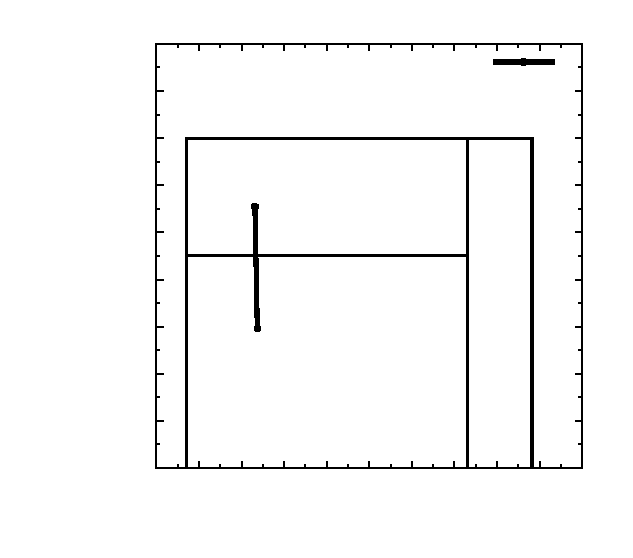
\includegraphics{/Users/kwh/sw_projects/hg/ft_program/wb/wb_chart}}%
    \gplfronttext
  \end{picture}%
\endgroup
